%********************************************************************************************************************************************************
\section[Statistical Framework]{Statistical Framework for Computer Model Analysis, Approximation, and Calibration}\label{sec:intro_statistical_framework}
%********************************************************************************************************************************************************

%-----------------------------------------------------------------------
\subsection[Sensitivity Analysis]{\Glsentryfull{sa}}\label{sub:intro_sa}
%-----------------------------------------------------------------------

An essential part of model development and assessment is 
properly describing and understanding the impact of model parameter variations on the model prediction.
\Gls{sa} is an important methodological step in that context \cite{Trucano2006}.
\gls{sa} is the process of investigating the role of input parameters in determining the model output \cite{Iooss2015}. 
It seeks to quantify the importance of each model input parameter on the output.

Various classifications exist in the literature to categorize \gls{sa} techniques \cite{Frey2002, Ionescu-Bujor2004, Cacuci2004, Saltelli2008, Iooss2015}.
In the review by Ionescu-Bujor and Cacuci \cite{Ionescu-Bujor2004, Cacuci2004}, 
\gls{sa} techniques are classified with respect to their scope (local vs. global) and to their framework (deterministic vs. statistical).
In the review of \gls{sa} methods by Iooss and Lemaître \cite{Iooss2015}, 
and the work by Saltelli et al. \cite{Saltelli2008} and by Santner et al. \cite{Santner2003}, 
the statistical framework is implicitly assumed deriving ideas from design of experiment, 
and the classification is based on the parameter space of interest (local vs. global).

Local analysis is based on calculating the effect on the model output of small perturbations around a nominal parameter value. 
\marginpar{local sensitivity analysis}
Often the perturbation is done one parameter at a time thus approximating the first-order partial derivative of the model output with respect to the perturbed parameter. 
The derivative can be computed through efficient adjoint formulation \cite{Cacuci2003,Cacuci2010} capable of handling large number of parameters.

Besides being numerically efficient, 
sensitivity coefficients obtained from local deterministic sensitivity analysis have the advantage of being intuitive in their interpretation, 
irrespective of the method employed \cite{Razavi2015}. 
The intuitiveness stems from the aforementioned equivalence to the derivative of the output with respect to each parameter \cite{Ionescu-Bujor2004} around a specifically defined point (i.e., nominal parameter values). 
Thus the coefficients can be readily compared over different modeled systems, 
independently of the range of parameters variations.

The global analysis, on the other hand, 
\marginpar{global sensitivity analysis}
seeks to explore the input parameters space across its range of variation 
and then quantify the input parameter importance based on a characterization of the resulting output response surface. 
In global deterministic framework \cite{Ionescu-Bujor2004,Cacuci2010}, 
the characterization is aimed at the identification of the system’s critical points (e.g., maxima, minima, saddle points, etc.). 
In statistical global methods \cite{Saltelli2008, Saltelli2004, Saltelli2006}, 
the characterization is aimed at measuring the dispersion of the output based on variance \cite{Sobol2001,Cukier1978}, 
correlation \cite{Helton1993}, or elementary effects \cite{Morris1991}.

Due to the different characterizations, 
the global statistical framework can potentially give spurious results not comparable to the results from local method 
as there is no unique definition of sensitivity coefficient provided by different global methods \cite{Razavi2015}. 
In some cases, different methods can give different and inconsistent parameters importance ranking \cite{Saltelli2008,Saltelli2004}. 
Furthermore, the result of the analysis can be highly dependent to the assumed input parameters probability distribution and/or their range of variation \cite{Cacuci2004,Cacuci2010}.

Yet, despite the aforementioned shortcomings, 
\marginpar{global statistical sensitivity analysis}
the global statistical framework has three particular attractive features relevant to the present study. 
First, the statistical method for sensitivity analysis is non-intrusive in the sense that minimal or no modification to the original code is required. 
In other words, the code can be taken as a black box and the analysis is focused on the input/output relationship \cite{Saltelli2008} of the code. 
This is the case especially in comparison to adjoint-based sensitivity \cite{Cacuci2000,Ionescu-Bujor2000} which is a highly efficient and accurate method applicable to a large number of parameters, 
provided that the code is designed/modified for adjoint analysis.

Second, no a priori knowledge on the model structure (linearity, additivity, etc.) is required. 
Depending on the model complexity and as the parameter variation range can be large, 
the linearity or additivity assumption might not hold.

Third and finally, 
the choice of a statistical framework for sensitivity analysis fits the Monte Carlo (MC)-based uncertainty propagation method widely adopted in nuclear reactor evaluation models \cite{Boyack1990, Nutt2004, Wallis2007, Glaeser2008}. 
The method prescribes that the uncertain model input and parameters (modeled as random variables) 
should be simultaneously and randomly perturbed across their range of variations. 
Multiple randomly generated input values are then propagated through the code to quantify the dispersion of the prediction (e.g., peak cladding temperature) 
which serves as a measure of the prediction reliability. 
Statistical global sensitivity analysis thus complements the propagation step 
by addressing the follow-up question on the identification of the most important parameters in driving the prediction uncertainty. 

Saltelli et al. \cite{Saltelli2006} emphasized that an analysis using computer simulation 
\marginpar{choosing model output as the quantity of interest}
should be focused on the specific question the simulation is required to answer 
as opposed to the analysis of each and every individual model output. 
This is done through judicious choice of representative quantity of interest (QoI) 
that properly substantiates the problem at hand. 
In particular, computer code output often comes in a form of time series. 
In such case, Saltelli et al. \cite{Saltelli2008,Saltelli2004} proposed to derive the relevant QoI from time-dependent output 
using a predefined scalar function such as the maximum, the minimum, the average, etc. that fits the initial question.

However, in some cases, the whole course of a transient is of primary interest 
\marginpar{function as model output}
such as in assessing the ability of a model to reproduce the overall dynamics of the simulated system. 
If the attention is focused on the overall change in shape of the time-dependent output (a shift in the Y-axis, a delay, a distortion, etc.), 
the descriptions provided by the aforementioned scalar functions might be incomplete and overlook important features of the variation. 
To tackle this problem, Campbell et al. \cite{Campbell2006} proposed to represent the functional (time-dependent) output in a certain basis function expansion 
and to carry out the sensitivity analysis on the coefficients of the expansion. 
In accordance to such approach, \gls{fda} popularized by Ramsay and Silverman \cite{Ramsay2005} can be useful to reduce the high dimensionality of time-dependent output.

% Recent Development in Nuclear Engineering Application
Despite these recent developments, 
\marginpar{recent development in nuclear engineering application}
there are very few publications on the application of global sensitivity analysis to nuclear thermal-hydraulics evaluation models specifically dealing with time-dependent output.
Notable recent examples related of sensitivity analysis for a time-dependent \gls{th} problem were the work done by Ionescu-Bujor et al. \cite{Ionescu-Bujor2005} 
for reflooding experiment of degraded fuel rods, utilizing adjoint sensitivity method; 
by Auder et al. \cite{Auder2012} for pressurized thermal shock analysis, 
utilizing statistical method with emphasis on metamodeling; 
and by Prošek and Leskovar \cite{Prosek2015} for \gls{lbloca} analysis, 
utilizing \gls{fftbm} and local sensitivity analysis.

\subsection{Bayesian Calibration}

\subsection{Statistical Metamodeling}\label{sub:intro_statistical_metamodeling}

% Why we need metamodel

% What is a metamodel

% Gaussian Process, What

% Gaussian Process, Why

% Gaussian Process, and others
\gls[hyper=false]{gp} metamodel is by no means the only method to construct a metamodel of a simulator, though it can be considered as the most popular choice in the literature (Table~\ref{tab:metamodel_in_literature}).
\marginpar{Other metamodeling approaches}
Response Surface Method (RSM), originally developed as a technique in the design and analysis of physical experiments \cite{Box2007}, 
has a long history of being adapted to the design and analysis of computer experiments \cite{Kerrigan1979,Lucia1982,Faravelli1989,Engel1990}.
It is mostly based on either linear or quadratic regression (with interaction terms) (see for instance cite \cite{Kleijnen2000}, and more recent reviews \cite{Simpson1998,Simpson2001}).
In recent times, other methods such as the ones based on artificial neural network \cite{Fonseca2003} and polynomial chaos expansion \cite{Sudret2008,Sudret2012} have also gained traction.
For comparison, Table~\ref{tab:metamodel_in_literature} shows the search hits from Scopus, an online bibliographic database \cite{Elsevier2017}, for the different select metamodeling approaches.

\begin{table}[ht]
    \myfloatalign
    \caption{Number of publications related to different metamodeling approaches based on Scopus web search as of Feb. $14$. $2017$.}
    \label{tab:metamodel_in_literature}
    \begin{tabularx}{\textwidth}{cXcc} \toprule
        \tableheadline{\footnotesize{Metamodeling}}	& \tableheadline{\footnotesize{Search}}\parnote{\texttt{(...) AND ("surrogate" OR "metamodel")}}  & \tableheadline{\footnotesize{Number of}}  & \tableheadline{\footnotesize{Since}} \\ 
				\tableheadline{\footnotesize{Approach}}     & \tableheadline{\footnotesize{Keyword}}  & \tableheadline{\footnotesize{Publications}}  &  \\ \midrule
        \multicolumn{1}{l}{\footnotesize{Gaussian Process / Kriging}} 		& \footnotesize{(\texttt{"Gaussian Process OR kriging"})}		& \footnotesize{$1838$} & \footnotesize{$1992$} \\
        \multicolumn{1}{l}{\footnotesize{Artificial Neural Network}}      & \footnotesize{\texttt{"neural network"}} 	 & \footnotesize{$997$} & \footnotesize{$1993$} \\
        \multicolumn{1}{l}{\footnotesize{Response Surface Method}}			  & \footnotesize{\texttt{"response surface"}} & \footnotesize{$947$} & \footnotesize{$1977$} \\
        \multicolumn{1}{l}{\footnotesize{Polynomial Chaos Expansion}}     & \footnotesize{\texttt{"polynomial chaos"}} & \footnotesize{$208$} & \footnotesize{$2004$} \\ \bottomrule
    \end{tabularx}
		\parnotes
\end{table}

% Recent development in nuclear engineering application
\lipsum[1]

\begin{sidewaysfigure}
	\centering
	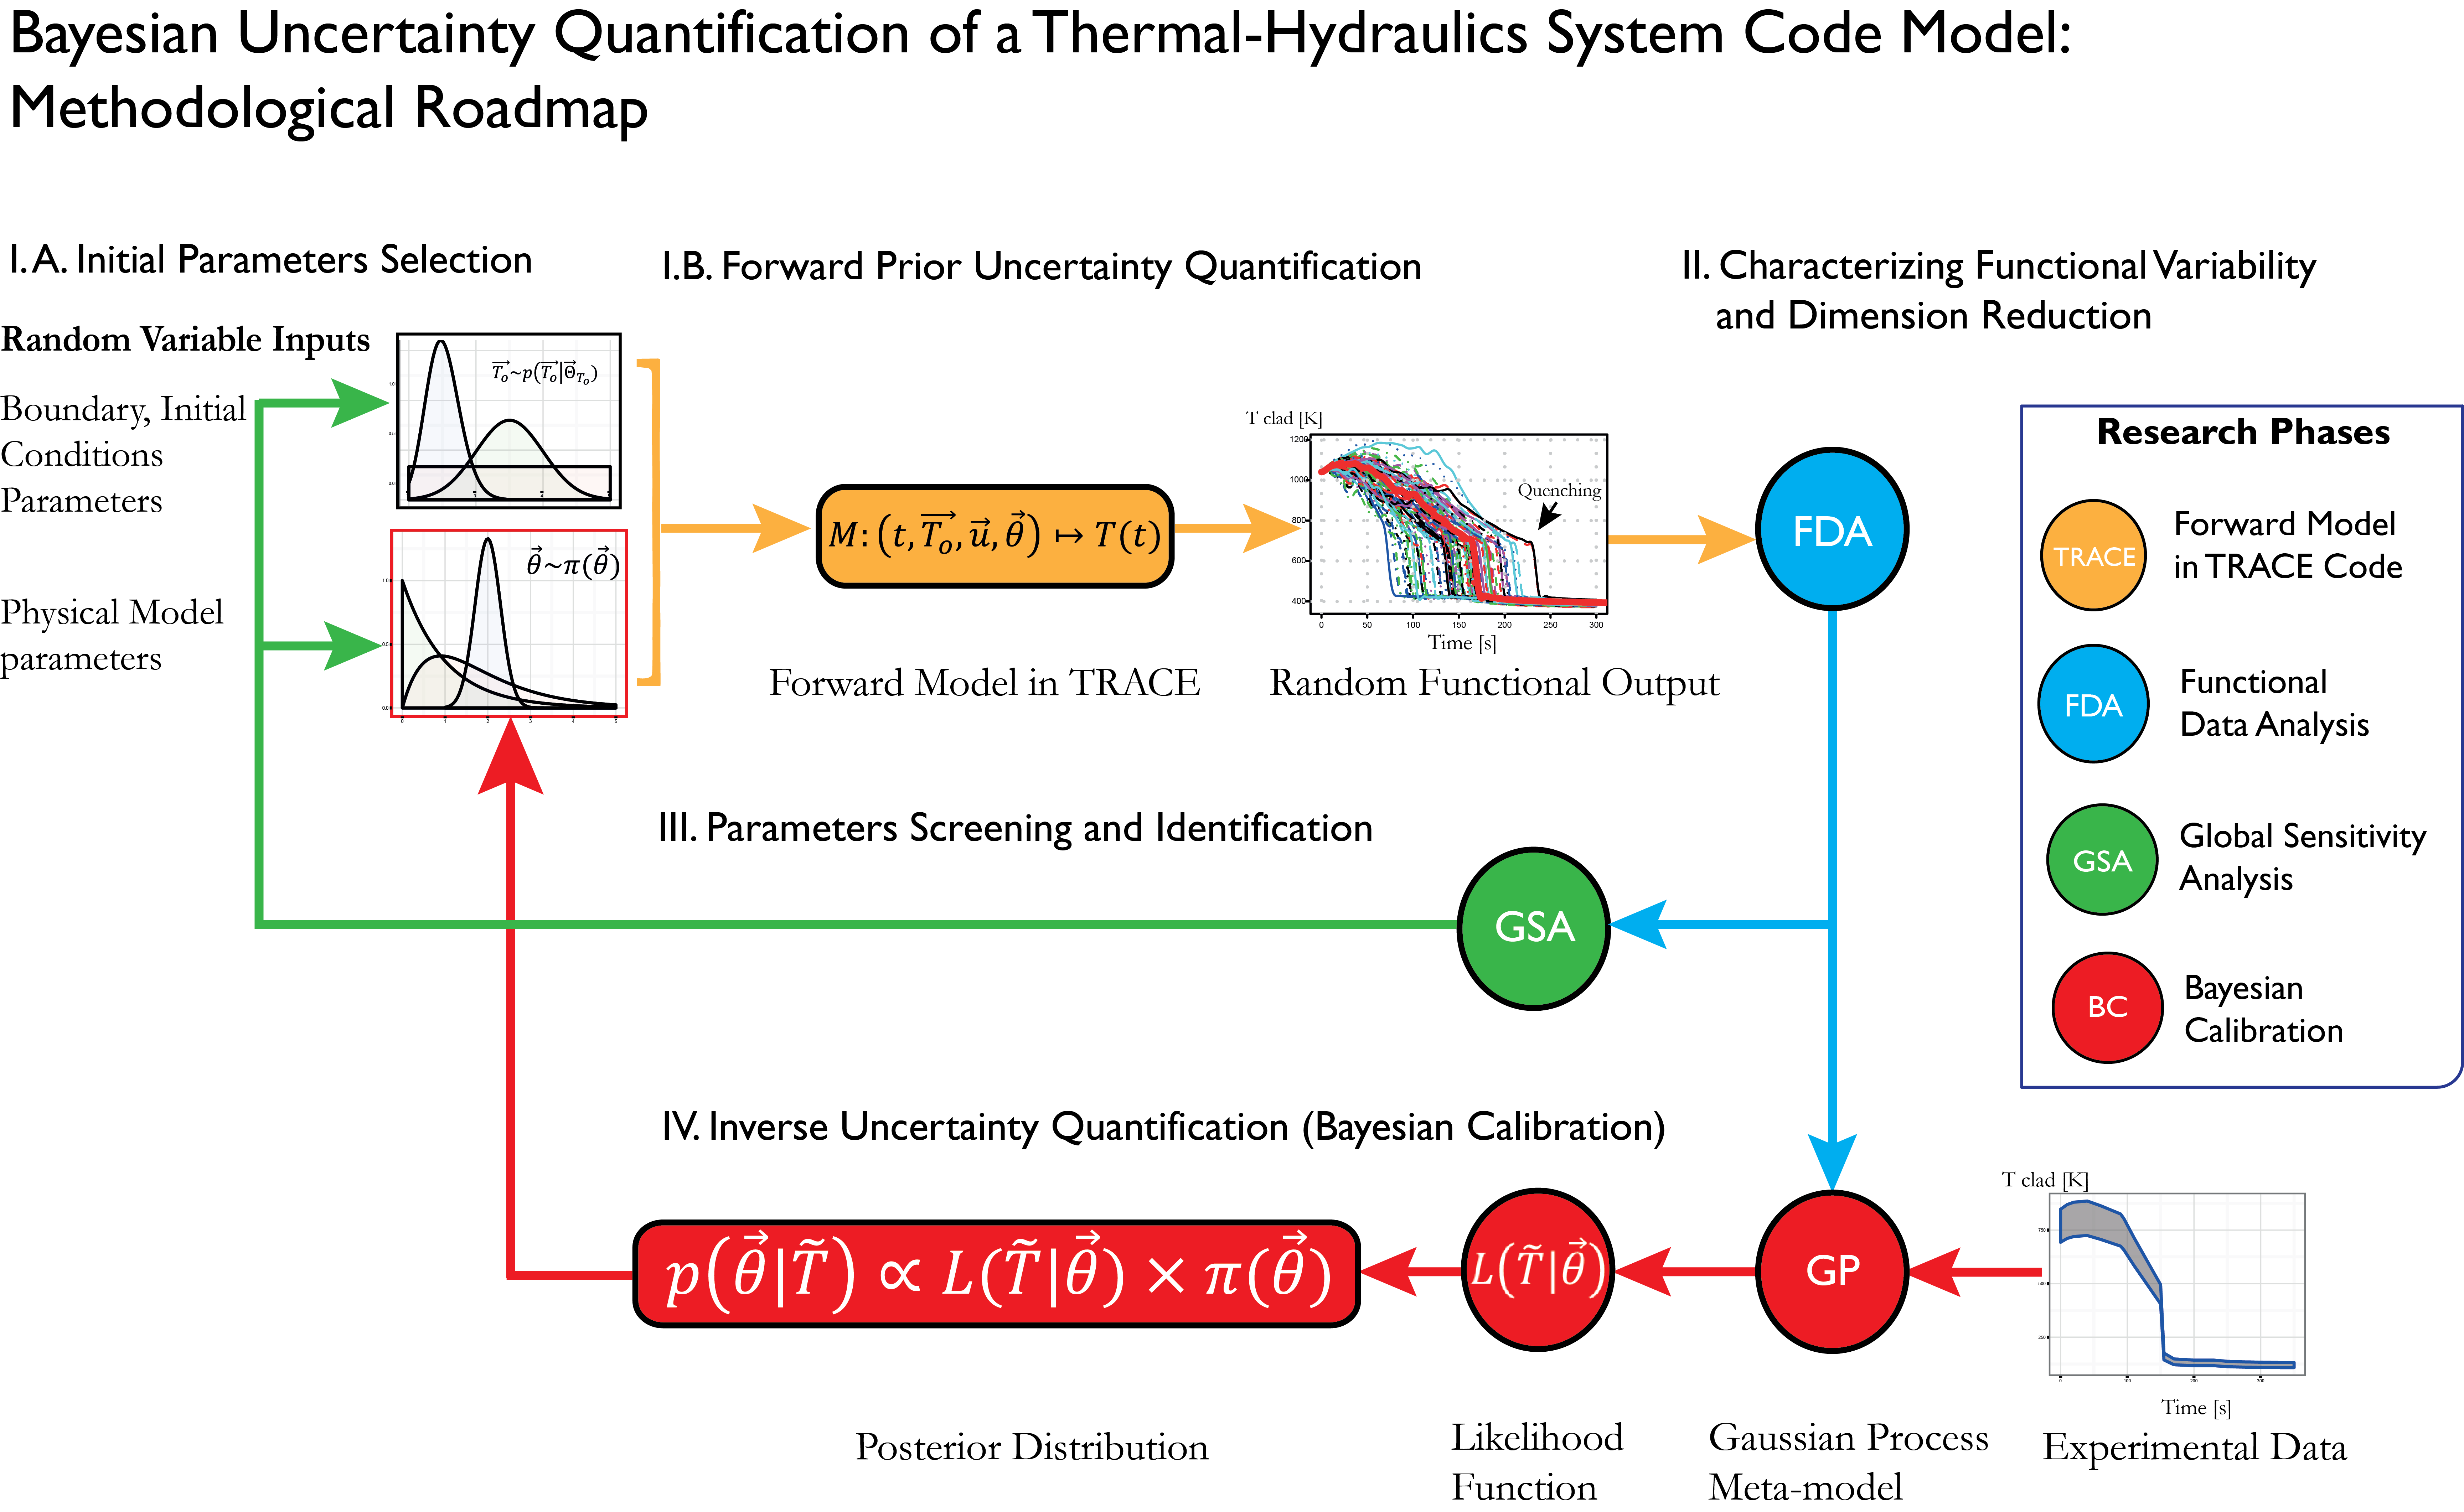
\includegraphics[width=0.85\textwidth]{../figures/methodologicalRoadmap/methodologicalRoadmap.pdf}
	\caption{Methodological Roadmap of the Thesis}
	\label{fig:methodological_roadmap}
\end{sidewaysfigure}
